\caulc
\begin{ex}%[2D4H1-3]%[TDMZZ20]%[Võ Hiệp]
	Họ nguyên hàm của hàm số $f(x)=\cos(\pi - x)$ là
	\choice
	{\True $-\sin x + C$}
	{$\sin x + C$}
	{$-\cos x + C$}
	{$\cos x + C$}
	\loigiai{
		Ta có $f(x)=\cos(\pi - x)= -\cos x$.\\
		Suy ra
		$\displaystyle\int\limits f(x) \mathrm{\,d}x=
		-\displaystyle\int\limits \cos x \mathrm{\,d}x=
		-\sin x + C$.
	}
\end{ex}

\begin{ex}%[2D4N3-4]%[TDMZZ20]%[Võ Hiệp]
	Cho vật thể X nằm dọc theo trục $Ox$, giới hạn bởi hai mặt phẳng vuông góc với $Ox$ tại các điểm $x=a$, $x=b$ ($a < b$). Một mặt phẳng vuông góc với $Ox$ tại điểm có hoành độ $x \in [a;b]$ cắt vật thể cho thiết diện có diện tích là hàm $S(x)$ liên tục trên đoạn $[a;b]$. Thể tích vật thể được tính là
	\choice
	{\True $V = \displaystyle\int\limits_a^b S(x)\mathrm{\,d}x$}
	{$V = \displaystyle\pi \int\limits_a^b S(x)\mathrm{\,d}x$}
	{$V = \pi \displaystyle\int\limits_a^b S^2(x)\mathrm{\,d}x$}
	{$V = \displaystyle\int\limits_a^b S^2(x)\mathrm{\,d}x$}
	\loigiai{
		Thể tích của vật thể X được tính bởi công thức
		$V = \displaystyle\int\limits_a^b S(x)\mathrm{\,d}x$.
	}
\end{ex}

\begin{ex}%[1D5H1-3]%[TDMZZ20]%[Võ Hiệp]
	Cho hai mẫu số liệu ghép nhóm $M_1$, $M_2$ với bảng tần số ghép nhóm
	\begin{center}
		\textbf{Nhóm $M_1$}\qquad
		\begin{tabular}{|c|c|c|c|c|c|}
			\hline
			Nhóm & $[3;4)$ & $[4;5)$ & $[5;6)$ & $[6;7)$ & $[7;8)$ \\ \hline
			Tần số & $3$ & $5$ & $4$ & $6$ & $2$ \\ \hline
		\end{tabular}
	\end{center}
	\begin{center}
		\textbf{Nhóm $M_2$}\qquad
		\begin{tabular}{|c|c|c|c|c|c|}
			\hline
			Nhóm & $[2;3)$ & $[3;4)$ & $[4;5)$ & $[5;6)$ & $[6;7)$ \\ \hline
			Tần số & $3$ & $3$ & $5$ & $4$ & $6$ \\ \hline
		\end{tabular}
	\end{center}
	Hãy so sánh số trung bình cộng $\overline{x}_1$, $\overline{x}_2$ của hai mẫu số liệu $M_1$, $M_2$?
	\choice
	{$\overline{x}_1 = 2\overline{x}_2$}
	{$\overline{x}_2 = 2\overline{x}_1$}
	{\True $\overline{x}_1 \,>\, \overline{x}_2$}
	{$\overline{x}_1 = \overline{x}_2$}
	\loigiai{
		Bảng tần số giá trị đại diện nhóm $M_1$
		\begin{center}
			\textbf{Nhóm $M_1$}\qquad
			\begin{tabular}{|c|c|c|c|c|c|}
				\hline
				Nhóm & $[3;4)$ & $[4;5)$ & $[5;6)$ & $[6;7)$ & $[7;8)$ \\ \hline
				Giá trị đại diện & $3{,}5$ & $4{,}5$ & $5{,}5$ & $6{,}5$ & $7{,}5$ \\ \hline
				Tần số & $3$ & $5$ & $4$ & $6$ & $2$ \\ \hline
			\end{tabular}
		\end{center}
		Số trung bình cộng của mẫu số liệu $M_1$ là
		\[\overline{x}_1 = \dfrac{3 \cdot 3{,}5 + 5 \cdot 4{,}5 + 4 \cdot 5{,}5 + 6 \cdot 6{,}5 + 2 \cdot 7{,}5}{3+5+4+6+2} = \dfrac{109}{20} = 5{,}45.\]
		Bảng tần số giá trị đại diện nhóm $M_2$
		\begin{center}
			\textbf{Nhóm $M_2$}\qquad
			\begin{tabular}{|c|c|c|c|c|c|}
				\hline
				Nhóm & $[2;3)$ & $[3;4)$ & $[4;5)$ & $[5;6)$ & $[6;7)$ \\ \hline
				Giá trị đại diện & $2{,}5$ & $3{,}5$ & $4{,}5$ & $5{,}5$ & $6{,}5$ \\ \hline
				Tần số & $3$ & $3$ & $5$ & $4$ & $6$ \\ \hline
			\end{tabular}
		\end{center}
		Số trung bình cộng của mẫu số liệu $M_2$ là
		\[\overline{x}_2 = \dfrac{3 \cdot 2{,}5 + 3 \cdot 3{,}5 + 5 \cdot 4{,}5 + 4 \cdot 5{,}5 + 6 \cdot 6{,}5}{3+3+5+4+6} = \dfrac{101{,}5}{21} \approx 4{,}83.\]
		Do đó $\overline{x}_1 \,>\, \overline{x}_2$.
	}
\end{ex}

\begin{ex}%[2H5N2-3]%[TDMZZ20]%[Võ Hiệp]
	Trong không gian $Oxyz$, phương trình tham số của trục $Oz$ là
	\choice
	{$\heva{&x=0 \\ &y=t \\ &z=0}$}
	{$\heva{&x=0 \\ &y=t \\ &z=t }$}
	{\True $\heva{&x=0 \\ &y=0 \\ &z=t}$}
	{$\heva{&x=t \\ &y=0 \\ &z=0}$}
	\loigiai{
		Trục $Oz$ đi qua gốc tọa độ $O(0;0;0)$ và có vectơ chỉ phương là $\overrightarrow{k} = (0;0;1)$.\\
		Do đó, phương trình tham số của trục $Oz$ là $\heva{&x=0 \\ &y=0 \\ &z=t.}$
	}
\end{ex}

\begin{ex}%[1D6H4-2]%[TDMZZ20]%[Võ Hiệp]
	Nghiệm của phương trình $\log\left(x^2-6\right)=1$ tương ứng là
	\choice
	{$\{\pm 2\}$}
	{$\{16\}$}
	{\True $\{\pm 4\}$}
	{$\{4\}$}
	\loigiai{
		Điều kiện xác định $x^2 - 6 > 0 \Leftrightarrow x^2 > 6 \Leftrightarrow \hoac{&x>\sqrt{6}\\& x<-\sqrt{6}.}$\\
		Khi đó
		\[\log(x^2-6)=1\Leftrightarrow x^2 - 6 = 10 \Leftrightarrow x^2 = 16 \Leftrightarrow x = \pm 4 \text{ (thỏa mãn)}.\]
		Vậy tập nghiệm của phương trình là $\{\pm 4\}$.
	}
\end{ex}

\begin{ex}%[2H5H2-3]%[TDMZZ20]%[Võ Hiệp]
	Trong không gian $Oxyz$, phương trình tổng quát của mặt phẳng $(\alpha)$ đi qua $A(1;2;2)$, có vectơ pháp tuyến $\overrightarrow{n}=(2;1;2)$ tương ứng là
	\choice
	{$(\alpha)\colon 2x+y+2z-5=0$}
	{\True $(\alpha)\colon 2x+y+2z-8=0$}
	{$(\alpha)\colon 2x+2y+z-8=0$}
	{$(\alpha)\colon x+2y+2z-8=0$}
	\loigiai{
		Phương trình mặt phẳng $(\alpha)$ đi qua $A(1;2;2)$ và có vectơ pháp tuyến $\overrightarrow{n}=(2;1;2)$ là
		\[2(x-1) + 1(y-2) + 2(z-2) = 0 \Leftrightarrow 2x+y+2z-8=0.\]
	}
\end{ex}

\begin{ex}%[2D1N5-1]%[TDMZZ20]%[Võ Hiệp]
	Cho hàm số $y = \dfrac{ax+b}{cx+d}$ ($c \neq 0, ad \neq bc$) có đồ thị như hình vẽ bên dưới.
	\begin{center}
		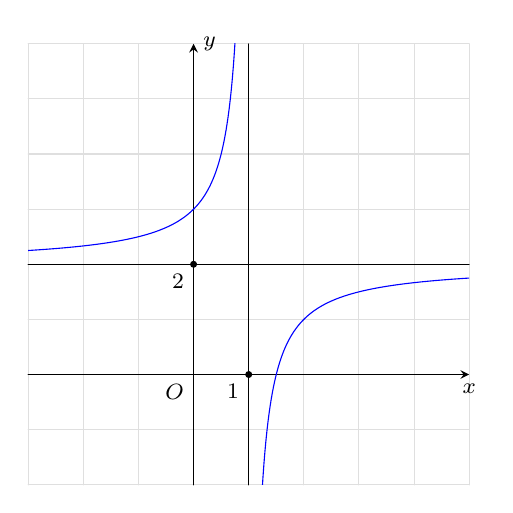
\begin{tikzpicture}[>=stealth,scale=0.7, font=\footnotesize, line join=round,line cap=round]
			% --- Thiết lập giới hạn khung hình ---
			\def\xmin{-3} \def\xmax{5}
			\def\ymin{-2} \def\ymax{6}
			% --- Lưới ô vuông ---
			\draw[gray!50,thin,opacity=.5] (\xmin,\ymin) grid (\xmax,\ymax);
			% --- Hệ trục tọa độ ---
			\draw[->] (\xmin,0)--(0,0)node[below left]{$O$}--(\xmax,0)node[below]{$x$};
			\draw[->] (0,\ymin)--(0,\ymax)node[right]{$y$};
			\draw (\xmin,2)--(\xmax,2) (1,\ymin)--(1,\ymax);
			\draw[fill] (1,0) circle (1.5pt) node[below left]{$1$};
			\draw[fill] (0,2) circle (1.5pt) node[below left]{$2$};
			% --- Vẽ đồ thị trong phạm vi clip ---
			\begin{scope}
				\clip (\xmin,\ymin) rectangle (\xmax,\ymax);
				\draw[blue, samples=200, domain=\xmin:0.8] plot (\x, {(2*\x-3)/(\x-1)});
				\draw[blue, samples=200, domain=1.2:\xmax] plot (\x, {(2*\x-3)/(\x-1)});
			\end{scope}
		\end{tikzpicture}
	\end{center}
	Tâm đối xứng của đồ thị hàm số đã cho là
	\choice
	{\True $(1;2)$}
	{$(2;1)$}
	{$(0;0)$}
	{$(0;2)$}
	\loigiai{
		Đồ thị hàm số có tiệm cận đứng là đường thẳng $x = 1$ và tiệm cận ngang là đường thẳng $y = 2$.\\
		Tâm đối xứng của đồ thị hàm số là giao điểm của hai đường tiệm cận, có tọa độ là $(1;2)$.
	}
\end{ex}

\begin{ex}%[1H8H2-3]%[TDMZZ20]%[Võ Hiệp]
	Cho hình chóp $S. ABCD$ có đáy $ABCD$ là hình chữ nhật, có $SA \perp (ABCD)$. Trong các cặp đường thẳng cho dưới đây, cặp nào \textbf{không} vuông góc với nhau?
	\choice
	{$SA$, $CD$}
	{$SC$, $BD$}
	{\True $SD$, $AC$}
	{$SA$, $BC$}
	\loigiai{
		\immini{
			\begin{itemize}
				\item Vì $SA \perp (ABCD)$ nên $SA \perp CD$ và $SA \perp BC$. Do đó, các cặp đường thẳng ở phương án A và D vuông góc với nhau.
				\item Xét phương án C: Hình chiếu vuông góc của $SD$ lên mặt phẳng $(ABCD)$ là $AD$. Vì $ABCD$ là hình chữ nhật nên $AD$ không vuông góc với $AC$. Theo định lý ba đường vuông góc, $SD$ không vuông góc với $AC$. Vậy cặp $SD$ và $AC$ là đáp án cần tìm.
				\item \textit{Lưu ý thêm:} Với phương án B, $SC$ và $BD$ chỉ vuông góc khi đáy $ABCD$ là hình vuông ($BD \perp AC$). Có thể đề bài gốc ngầm giả định đáy là hình vuông, tuy nhiên dù đáy là hình vuông hay hình chữ nhật thì cặp $SD$ và $AC$ vẫn luôn không vuông góc với nhau.
			\end{itemize}
		}{
			\begin{tikzpicture}[scale=1,>=stealth, font=\footnotesize, line join=round, line cap=round]
				\def\a{3}
				\def\h{3}
				\path 	(0:0) coordinate (A)
				++(0:\a) coordinate (D)
				++(-130:\a/2) coordinate (C)
				($(A)+(C)-(D)$) coordinate (B)
				($(A)+(90:\h)$) coordinate (S)
				(intersection of A--C and B--D) coordinate (O);
				\draw[dashed,thick] 	(B)--(A)--(D)	(A)--(S) (A)--(C) (B)--(D);
				\draw[thick] 			(B)-- (C)--(D)
				(B)--(S)	(C)--(S)	(D)--(S);
				\foreach \x/\g in {A/135,B/-135,C/-45,D/45,S/90}
				\fill[black] 	(\x) circle (1.5pt)
				($(\g:3mm)+(\x)$) node {$\x$};	
			\end{tikzpicture}
		}
	}
\end{ex}

\begin{ex}%[1D7N2-1]%[TDMZZ20]%[Võ Hiệp]
	Biểu thức đạo hàm của hàm số $y = 3^x$ là
	\choice
	{$y' = 3^x$}
	{$y' = \dfrac{3^x}{\ln 3}$}
	{\True $y' = 3^x \ln 3$}
	{$y' = \dfrac{3^x}{\ln 3} + 2026$}
	\loigiai{
		Ta có $y' = \left(3^x\right)' = 3^x \ln 3$.
	}
\end{ex}

\begin{ex}%[1D2N2-4]%[TDMZZ20]%[Võ Hiệp]
	Cho cấp số cộng $(u_n)$ có $u_1 = 7$ và công sai $d = -2$. Số hạng $u_3$ bằng
	\choice
	{$1$}
	{$5$}
	{\True $3$}
	{$28$}
	\loigiai{
		Ta có $u_3 = u_1 + 2d = 7 + 2 \cdot (-2) = 3$.
	}
\end{ex}

\begin{ex}%[2H2H1-2]%[TDMZZ20]%[Võ Hiệp]
	\immini[thm]{	Cho hình hộp $ABCD. A'B'C'D'$. Hỏi phát biểu nào dưới đây \textbf{đúng}?
		
		\choice
		{$\overrightarrow{AB} + \overrightarrow{AC} + \overrightarrow{AA'} = \overrightarrow{AC'}$}
		{$\overrightarrow{AB} + \overrightarrow{A'D} + \overrightarrow{AA'} = \overrightarrow{AC'}$}
		{\True $\overrightarrow{AB} + \overrightarrow{A'D'} + \overrightarrow{CC'} = \overrightarrow{AC'}$}
		{$\overrightarrow{AB} + \overrightarrow{A'D} + \overrightarrow{AA'} = \overrightarrow{AC'}$}
	}{
		\begin{tikzpicture}[scale=0.8, line join=round, line cap=round, >=stealth, font=\footnotesize]
			\def\a{3} \def\b{2} \def\g{80}
			\path 
			(0,0) coordinate (A) ++ (0:\a) coordinate (B)++ (60:\b) coordinate (C)
			($(A)+(C)-(B)$) coordinate (D)
			(A)++(\g:\a) coordinate (A') ++ (0:\a) coordinate (B')++ (60:\b) coordinate (C')
			($(A')+(C')-(B')$) coordinate (D')
			;
			
			\draw[dashed] (A) -- (D) -- (C);
			\draw[dashed] (D) -- (D');
			\draw (A) -- (B) -- (C) -- (C') -- (D') -- (A') -- (A);
			\draw (B) -- (B') -- (C');
			\draw (A') -- (B');
			\foreach \diem/\goc in {A/-150, B/-30, C/-45, D/-45, A'/150,B'/-40,C'/30,D'/150}
			\fill[black] (\diem) circle (1.5pt) ++(\goc:0.3) node{$\diem$};
		\end{tikzpicture}
	}
	\loigiai{
		Vì $ABCD. A'B'C'D'$ là hình hộp nên ta có $\overrightarrow{A'D'} = \overrightarrow{AD}$, $\overrightarrow{CC'} = \overrightarrow{AA'}$.\\
		Áp dụng quy tắc hình hộp, ta có
		\[\overrightarrow{AB} + \overrightarrow{A'D'} + \overrightarrow{CC'} = \overrightarrow{AB} + \overrightarrow{AD} + \overrightarrow{AA'} = \overrightarrow{AC'}.\]
	}
\end{ex}

\begin{ex}%[2D1H4-3]%[2D1H4-4]%[TDMZZ20]%[Võ Hiệp]
	Đồ thị của hàm số $y = \dfrac{x^2-3x+4}{x-2}$
	\choice
	{không có cực trị}
	{đồng biến trên từng khoảng xác định}
	{\True có tâm đối xứng là điểm $(2;1)$}
	{nghịch biến trên từng khoảng xác định}
	\loigiai{
		Ta có $y = \dfrac{x^2-3x+4}{x-2} = x - 1 + \dfrac{2}{x-2}$.\\
		Tập xác định $\mathcal{D} = \mathbb{R} \setminus \{2\}$.\\
		Đạo hàm $y' = 1 - \dfrac{2}{(x-2)^2} = \dfrac{(x-2)^2-2}{(x-2)^2}$.\\
		Cho $y' = 0 \Leftrightarrow (x-2)^2 = 2 \Leftrightarrow x = 2 \pm \sqrt{2}$.\\
		Bảng biến thiên
		\begin{center}
			
\begin{tikzpicture}[scale=0.8, line join=round, line cap=round, >=stealth, font=\footnotesize]	 
				\tkzTabInit[nocadre=true,lgt=1,espcl=2.5,deltacl=0.6]
				{$x$/.7, $y' $/.7, $y $/2.2}	
				{$-\infty$,$2-\sqrt{2}$,$2$,$2+\sqrt{2}$,$+\infty$}
				\tkzTabLine{,+,0,-,d,-,0,+,} %h là tô nền
				\tkzTabVar{-/$-\infty$,+/$1-2\sqrt{2}$, -D+/$-\infty$/$+\infty$,-/$1+2\sqrt{2}$,+/$+\infty$}
			\end{tikzpicture}
		\end{center}
		Từ bảng biến thiên suy ra
		\begin{itemize}
			\item Hàm số đã cho có $2$ điểm cực trị.
			\item Hàm số đồng biến trên khoảng $\left(-\infty; 2-\sqrt{2}\right)$ và $\left(2+\sqrt{2}; +\infty\right)$.
			\item Hàm số nghịch biến trên khoảng $\left(2-\sqrt{2};2\right)$ và $\left(2; 2+\sqrt{2}\right)$.
			\item Ta có
			\begin{itemize}
				\item $\lim\limits_{x\to 2^-}\dfrac{x^2-3x+4}{x-2}=-\infty$ và $\lim\limits_{x\to 2^+}\dfrac{x^2-3x+4}{x-2}=+\infty$, suy ra tiệm cận đứng là $x = 2$.
				\item $\lim\limits_{x\to \pm\infty}\left[y-(x-1)\right]= \lim\limits_{x\to \pm\infty}\dfrac{2}{x-2}=0$, suy ra tiệm cận xiên $y=x-1$.
			\end{itemize}
			Do đó giao điểm của hai đường tiệm cận là $I(2;1)$, đây chính là tâm đối xứng của đồ thị hàm số.
		\end{itemize}
	}
\end{ex}
\cauds
\begin{ex}%[2D1H2-1]%[Dương Công Tạo]
	Trong mặt phẳng toạ độ $Oxy$, cho hàm số $y = f(x) = x^4 - 8x^2 + 7$ có đồ thị $(C)$.
	\choiceTF
	{\True $f'(x) = 4x^3-16x$}
	{\True Hàm số $f(x)$ có ba điểm cực trị}
	{\True Ba điểm cực trị của $(C)$ tạo thành một tam giác cân}
	{Diện tích của tam giác tạo bởi ba điểm cực trị là $4\sqrt{3}$}
	\loigiai{
		\begin{itemchoice}
			\itemch Xét hàm số $y = f(x) = x^4 - 8x^2 + 7$.\\
			Tập xác định $\mathscr{D}=\mathbb{R}$.\\
			Ta có $f'(x) = 4x^3-16x$.
			\itemch $f'(x)=0 \Leftrightarrow 4x^3-16x=0 \Leftrightarrow \hoac{&x=0\\&x=\pm 2}$.\\
			Bảng biến thiên
			\begin{center}
				
\begin{tikzpicture}
					\tkzTabInit[nocadre=true, lgt=1.2, espcl=2.5, deltacl=0.5]
					{$x$ /0.7, $f'(x)$ /0.7, $f(x)$ /2}
					{$-\infty$, $-2$, $0$, $2$, $+\infty$}
					\tkzTabLine{, -, 0, +, 0, -, 0, +, }
					\tkzTabVar{+/ $+\infty$, -/ $-9$, +/ $7$, -/ $-9$, +/ $+\infty$}
				\end{tikzpicture}
			\end{center}
			Dựa vào bảng biến thiên, hàm số $f(x)$ có $3$ điểm cực trị.
			\itemch Gọi $A(0;7)$, $B(2;-9)$ và $C(-2;-9)$ là ba điểm cực trị của $(C)$.\\
			Ta có $A \in Oy$ và $B, C$ đối xứng nhau qua trục $Oy$ (do hàm số chẵn).\\
			Nên $\triangle ABC$ cân tại đỉnh $A$.
			\itemch Gọi $H$ là trung điểm $BC$, ta có $H(0;-9)$.\\
			Khi đó $AH = |y_A - y_H| = 7 - (-9) = 16$.\\
			Độ dài cạnh đáy $BC = |x_C - x_B| = |-2 - 2| = 4$.\\
			Diện tích $\triangle ABC$ là $S_{ABC} = \dfrac{1}{2} \cdot BC \cdot AH = \dfrac{1}{2} \cdot 4 \cdot 16 = 32$.
		\end{itemchoice}
	}
\end{ex}

\begin{ex}%[TDMZZ20]%[Hà Văn Hảo]%[2D6V2-3]
	Cho hộp I có đựng $6$ viên bi đỏ và $8$ viên bi xanh, các viên bi có cùng kích thước và cùng khối lượng, hộp II ban đầu chưa đựng gì. Hải lấy ngẫu nhiên một viên bi từ hộp I để bỏ vào hộp II, sau đó Dũng nhìn vào hộp II để quan sát, nếu thấy viên bi màu đỏ thì Dũng lấy ngẫu nhiên từ hộp I ra hai viên bi bỏ vào hộp II, còn nếu thấy viên bi màu xanh thì Dũng lấy ngẫu nhiên từ hộp I ra một viên bi bỏ vào hộp II. Gọi $A$ là biến cố Hải lấy được bi màu đỏ, $B$ là biến cố các viên bi ở hộp II cùng màu (tính từ thời điểm sau khi Dũng đã lấy xong bi ở hộp I để bỏ vào hộp II).
	\choiceTF
	{\True $\mathrm{P}(A) = \dfrac{3}{7}$}
	{\True Xác suất để hộp II có hai viên bi (sau khi Dũng đã lấy bỏ vào) là $\dfrac{4}{7}$}
	{\True $\mathrm{P}(B \mid A) = \dfrac{5}{39}$}
	{ $\mathrm{P}(A \mid B) = \dfrac{2}{5}$}
	\loigiai{
		Hộp I ban đầu có $14$ viên bi ($6$ đỏ, $8$ xanh).
		\begin{itemchoice}
			\itemch Biến cố $A$ là Hải lấy được $1$ viên bi đỏ từ hộp I.\\
			Số cách chọn $1$ viên bi từ $14$ viên là $n(\Omega_1) = \mathrm{C}_{14}^1 = 14$.\\
			Số cách chọn $1$ viên bi đỏ là $n(A) = \mathrm{C}_6^1 = 6$.\\
			Xác suất $\mathrm{P}(A) = \dfrac{6}{14} = \dfrac{3}{7}$.
			\itemch Gọi $E$ là biến cố hộp II có hai viên bi sau khi Dũng lấy xong.\\
			Hộp II có hai viên bi khi và chỉ khi Dũng lấy thêm $1$ viên bi, điều này xảy ra khi Hải lấy được bi màu xanh (biến cố $\overline{A}$).\\
			Xác suất $\mathrm{P}(E) = \mathrm{P}(\overline{A}) = 1 - \mathrm{P}(A) = 1 - \dfrac{3}{7} = \dfrac{4}{7}$.
			\itemch Khi biến cố $A$ đã xảy ra: Hải đã lấy $1$ viên bi đỏ bỏ vào hộp II. Hộp I còn lại $5$ đỏ và $8$ xanh (tổng $13$ viên).\\
			Dũng thấy bi đỏ nên lấy thêm $2$ viên từ hộp I bỏ vào hộp II.\\
			Để các viên bi trong hộp II cùng màu (biến cố $B$), Dũng phải lấy thêm $2$ viên bi đỏ từ $13$ viên còn lại trong hộp I.\\
			Xác suất có điều kiện $\mathrm{P}(B \mid A) = \dfrac{\mathrm{C}_5^2}{\mathrm{C}_{13}^2} = \dfrac{10}{78} = \dfrac{5}{39}$.
			\itemch Ta tính xác suất của biến cố $B$ bằng công thức xác suất toàn phần
			\[\mathrm{P}(B) = \mathrm{P}(A) \cdot \mathrm{P}(B \mid A) + \mathrm{P}(\overline{A}) \cdot \mathrm{P}(B \mid \overline{A}).\]
			Nếu $\overline{A}$ xảy ra: Hải lấy $1$ bi xanh, hộp I còn $6$ đỏ và $7$ xanh.\\
			Dũng lấy thêm $1$ viên. Để cùng màu (xanh), Dũng phải lấy $1$ bi xanh từ $13$ viên.
			\allowdisplaybreaks
			\begin{eqnarray*}
				&\mathrm{P}(B \mid \overline{A}) = \dfrac{\mathrm{C}_7^1}{\mathrm{C}_{13}^1} = \dfrac{7}{13}.\\
				&\mathrm{P}(B) = \dfrac{3}{7} \cdot \dfrac{5}{39} + \dfrac{4}{7} \cdot \dfrac{7}{13} = \dfrac{5}{91} + \dfrac{28}{91} = \dfrac{33}{91}.
			\end{eqnarray*}
			Theo công thức Bayes
			$\mathrm{P}(A \mid B) = \dfrac{\mathrm{P}(A \cap B)}{\mathrm{P}(B)} = \dfrac{\mathrm{P}(A) \cdot \mathrm{P}(B \mid A)}{\mathrm{P}(B)} = \dfrac{\frac{5}{91}}{\frac{33}{91}} = \dfrac{5}{33}$.
		\end{itemchoice}
	}
\end{ex}

\begin{ex}%[2D4V3-1]%[TDMZZ20]%[Vũ Hồng Toàn]
	Trong mặt phẳng tọa độ $Oxy$, cho đường tròn $(C)$ có tâm $I(0;5)$ và bán kính $R$ và một đường parabol tiếp xúc với $(C)$ như hình vẽ. Gọi $(H)$ là phần hình phẳng được tô màu như hình vẽ. Gọi phương trình nửa đường tròn của $(C)$ nằm dưới đường thẳng $y=5$ là $y=f(x)$ và phương trình parabol là $y=g(x)=ax^2+bx+c$.
	\begin{center}
		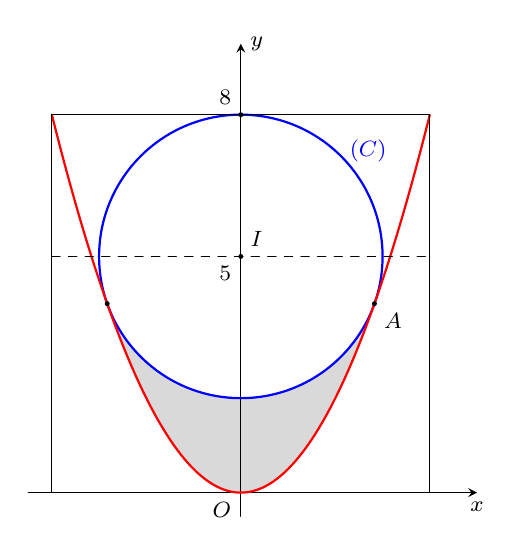
\begin{tikzpicture}[scale=0.6, font=\footnotesize, line join=round, line cap=round, >=stealth]
			% Tô màu phần hình phẳng H
			\fill[gray!30] plot[domain=-2.828:2.828, samples=100] (\x, {0.5*(\x)^2}) -- plot[domain=2.828:-2.828, samples=100] (\x, {5 - sqrt(9 - (\x)^2)}) -- cycle;
			
			% Vẽ hệ trục tọa độ
			\draw[->] (-4.5,0) -- (5,0) node[below] {$x$};
			\draw[->] (0,-0.5) -- (0,9.5) node[right] {$y$};
			\node[below left] at (0,0) {$O$};
			
			% Vẽ đường tròn (C)
			\draw[blue, thick] (0,5) circle (3);
			\node[blue, above right] at (2.1, 6.8) {$(C)$};
			
			% Vẽ parabol
			\draw[red, thick, domain=-4:4, samples=100] plot (\x, {0.5*(\x)^2});
			
			% Vẽ đường thẳng nét đứt y = 5
			\draw[dashed] (-4,5) -- (4,5);
			
			% Các điểm đặc biệt
			\fill (0,5) circle (1.5pt) node[above right] {$I$} node[below left] {$5$};
			\fill (0,8) circle (1.5pt) node[above left] {$8$};
			\fill (2.828,4) circle (1.5pt) node[below right] {$A$};
			\fill (-2.828,4) circle (1.5pt);
			
			% Khung hình chữ nhật bao quanh
			\draw (-4,0) -- (-4,8) -- (4,8) -- (4,0);
		\end{tikzpicture}
	\end{center}
	Biết rằng điều kiện để hai đường cong $y=f(x)$ và $y=g(x)$ tiếp xúc với nhau tại một điểm $(x_0;y_0)$ thì phải thỏa mãn hệ phương trình tiếp điểm $\heva{&f'(x_0)=g'(x_0) \\& f(x_0)=g(x_0).}$
	\choiceTF
	{Phương trình đường tròn $(C)$ là $x^2+(y-5)^2=64$}
	{\True Ta có $b=c=0$, tức là $y=g(x)=ax^2$}
	{\True $y=f(x)=5-\sqrt{9-x^2}$}
	{Diện tích hình phẳng $(H)$ bằng $4{,}32$ (làm tròn kết quả đến hàng đơn vị)}
	\loigiai{
		\begin{itemchoice}
			\itemch Dựa vào hình vẽ, đường tròn $(C)$ có tâm $I(0;5)$ và đi qua điểm có tung độ bằng $8$ trên trục $Oy$. Do đó bán kính của đường tròn là $R = 8 - 5 = 3$.\\
			Phương trình đường tròn $(C)$ là $x^2 + (y-5)^2 = 9$.
			\itemch Parabol $(P) \colon y = g(x) = ax^2 + bx + c$ đi qua gốc tọa độ $O(0;0)$ nên $g(0) = c = 0$.\\
			Mặt khác, parabol nhận trục tung (đường thẳng $x=0$) làm trục đối xứng nên $-\dfrac{b}{2a}=0 \Leftrightarrow b=0$.\\
			Do đó phương trình parabol là $y = g(x) = ax^2$.
			\itemch Từ phương trình đường tròn $x^2 + (y-5)^2 = 9 \Rightarrow (y-5)^2 = 9 - x^2 \Rightarrow y = 5 \pm \sqrt{9-x^2}$.\\
			Vì nửa đường tròn nằm dưới đường thẳng $y=5$ nên phương trình của nó là \[y = f(x) = 5 - \sqrt{9-x^2}.\]
			\itemch Ta có $f'(x) = \dfrac{x}{\sqrt{9-x^2}}$ và $g'(x) = 2ax$. Xét hệ phương trình tiếp điểm của hai đường cong tại điểm có hoành độ $x_0 > 0$:
			\[\heva{&f'(x_0) = g'(x_0) \\& f(x_0) = g(x_0)}\Leftrightarrow\heva{&\dfrac{x_0}{\sqrt{9-x_0^2}} = 2ax_0 \quad&(1)\\& 5 - \sqrt{9-x_0^2} = ax_0^2.\quad &(2)}\]
			Vì $x_0 > 0$ nên từ phương trình $(1)$ ta có
			\[2a = \dfrac{1}{\sqrt{9-x_0^2}} \Rightarrow a = \dfrac{1}{2\sqrt{9-x_0^2}}.\]
			Thay vào phương trình $(2)$ ta được
			\[5 - \sqrt{9-x_0^2} = \dfrac{x_0^2}{2\sqrt{9-x_0^2}} \Leftrightarrow 10\sqrt{9-x_0^2} - 2(9-x_0^2) = x_0^2.\quad (*)\]
			Đặt $t = \sqrt{9-x_0^2}$ ($0 < t < 3$) $\Rightarrow x_0^2 = 9 - t^2$. Phương trình $(*)$ trở thành
			\[10t - 2t^2 = 9 - t^2 \Leftrightarrow t^2 - 10t + 9 = 0 \Leftrightarrow\hoac{&t = 1 &\text{ (nhận)} \\& t = 9 &\text{ (loại)}.}\]
			Với $t = 1 \Rightarrow \sqrt{9-x_0^2} = 1 \Rightarrow x_0^2 = 8 \Rightarrow x_0 = 2\sqrt{2}$ (do $x_0 > 0$).\\
			Suy ra $a = \dfrac{1}{2\cdot 1} = \dfrac{1}{2}$.\\
			Do đó phương trình parabol là $y = g(x) = \dfrac{1}{2}x^2$.\\
			Do tính đối xứng qua $Oy$, diện tích hình phẳng $(H)$ giới hạn bởi hai đường cong là
			\[S = 2 \displaystyle\int\limits_0^{2\sqrt{2}} \left[ \left(5 - \sqrt{9-x^2}\right) - \dfrac{1}{2}x^2 \right] \mathrm{\,d}x \approx 6{,}83.\]
			Vậy mệnh đề sai.
		\end{itemchoice}
	}
\end{ex}

\begin{ex}%[2H5V3-4]%[TDMZZ20]%[Văn Minh Thoại]
	Trong không gian $Oxyz$ có đơn vị dài trên mỗi trục là centimet, có một quả cầu nhỏ có bán kính bằng $20$ cm, ở thời điểm ban đầu $t_0=0$ tâm của nó ở vị trí $I_0(0;0;0)$ và có một sợi dây căng đủ dài nằm trên đường thẳng $d\colon\heva{&x=70\\&y=t'\\&z=t'}$. Quả cầu nhỏ bắt đầu chuyển động tịnh tiến với tốc độ bằng $v=15$ cm/s theo hướng vectơ $\overrightarrow{u}=(1;2;2)$.
	\choiceTF
	{\True Quả cầu nhỏ va chạm vào dây nếu khoảng cách từ tâm quả cầu đến sợi dây đúng bằng bán kính quả cầu}
	{Ở thời điểm $t$, tâm của quả cầu ở vị trí $I$ thoả mãn $\overrightarrow{I_0I}=t\overrightarrow{u}$, với $t\ge 0$}
	{Khoảng cách từ tâm quả cầu đến sợi dây ở thời điểm $t$ là $|t-70|$}
	{\True Sau đúng $10$ giây tính từ thời điểm quả cầu bắt đầu chuyển động thì quả cầu va vào sợi dây}
	\loigiai{
		\begin{itemchoice}
			\itemch Quả cầu nhỏ va chạm vào dây nếu khoảng cách từ tâm quả cầu đến sợi dây đúng bằng bán kính quả cầu $\mathrm{d}\big(I, d\big)=R=20$ (trường hợp tiếp xúc). 
			\itemch Quả cầu chuyển động với tốc độ $v=15$ cm/s theo hướng của vectơ $\overrightarrow{u}=(1;2;2)$. \\
			Độ dài của $\overrightarrow{u}$ là $\left|\overrightarrow{u}\right|=\sqrt{1^2+2^2+2^2}=3$. \\
			Vectơ vận tốc $\overrightarrow{v}$ cùng hướng với $\overrightarrow{u}$ và có độ lớn $15$, do đó
			\[\overrightarrow{v} = \dfrac{15}{\left|\overrightarrow{u}\right|} \overrightarrow{u} = \dfrac{15}{3} \overrightarrow{u} = 5\overrightarrow{u}.\]
			Quãng đường tịnh tiến của tâm quả cầu sau thời gian $t$ ($t\ge 0$) là
			\[\overrightarrow{I_0I} = \overrightarrow{v}t = 5t\overrightarrow{u}.\]
			\itemch Đường thẳng $d\colon\heva{&x=70\\&y=t'\\&z=t'}$ đi qua điểm $A(70;0;0)$ và có vectơ chỉ phương $\overrightarrow{u}_d=(0;1;1)$. \\
			Tại thời điểm $t$, tâm quả cầu là $I(5t; 10t; 10t)$. \\
			Ta có vectơ $\overrightarrow{AI}=(5t-70; 10t; 10t)$. \\
			Suy ra
			\[\left[\overrightarrow{AI}, \overrightarrow{u}_d\right] = \left( \begin{vmatrix} 10t & 10t \\ 1 & 1
			\end{vmatrix}; \begin{vmatrix} 10t & 5t-70 \\ 1 & 0
			\end{vmatrix};	\begin{vmatrix} 5t-70 & 10t \\ 0 & 1
			\end{vmatrix} \right) = (0; 70-5t; 5t-70)\]
			Khoảng cách từ tâm $I$ đến sợi dây $d$ tại thời điểm $t$ là
			\[d(I,d) = \dfrac{\left| \left[\overrightarrow{AI}, \overrightarrow{u}_d\right] \right|}{\left|\overrightarrow{u}_d\right|} = \dfrac{\sqrt{0^2 + (70-5t)^2 + (5t-70)^2}}{\sqrt{0^2 + 1^2 + 1^2}} = \dfrac{\sqrt{2(5t-70)^2}}{\sqrt{2}} = |5t-70|.\]
			Khoảng cách tính được là $|5t-70|\neq |t-70|$. 
			\itemch Quả cầu bắt đầu va chạm vào sợi dây khi khoảng cách từ tâm đến dây bằng bán kính $R=20$ cm. \\
			Ta có phương trình
			\allowdisplaybreaks
			\begin{align*}
				\mathrm{d}\big(I,d\big) = 20 &\Leftrightarrow |5t-70| = 20 \\
				&\Leftrightarrow \hoac{&5t-70 = 20 \\ &5t-70 = -20} \\
				&\Leftrightarrow \hoac{&5t = 90 \\ &5t = 50} \\
				&\Leftrightarrow \hoac{&t = 18 \\ &t = 10.}
			\end{align*}
			Thời điểm bắt đầu va chạm ứng với $t$ nhỏ hơn, tức là $t=10$ (giây).\\
			Vậy sau đúng $10$ giây quả cầu va vào sợi dây. 
			\begin{center}
				\begin{tikzpicture}[declare function={R=1.5; sina=1/3; cosa=sqrt (8)/3; D=4.5; xA=-D*cosa; yA=-D*sina; xB=0; yB=0; xC=D*cosa; yC=D*sina; len=6.5;},line join=round,line cap=round,>=stealth,scale=0.7]
					\path
					(xA,yA) coordinate (IA)
					(xB,yB) coordinate (IB)
					(xC,yC) coordinate (IC)
					(xA,0) coordinate (HA)
					(xC,0) coordinate (HC)
					(-len,0) coordinate (D1)
					(len,0) coordinate (D2)
					(-len*cosa,-len*sina) coordinate (Delta1)
					(len*cosa,len*sina) coordinate (Delta2);
					\draw (D1) -- (D2) node[pos=0.95,sloped,above] {$d$};
					\draw[fill=cyan!10] (IA) circle (R);
					\draw[fill=cyan!10] (IB) circle (R);
					\draw[fill=cyan!10] (IC) circle (R);
					\draw[dashed,->] (Delta1) -- (Delta2) node[pos=0.92,sloped,above] {$\Delta$};
					\draw[dashed] (IA) -- (HA) node[pos=0.5,left] {$R$};
					\draw[dashed] (IC) -- (HC) node[pos=0.5,right] {$R$};
					\path pic[draw,angle radius=5pt]{right angle=IA--HA--IB};
					\path pic[draw,angle radius=5pt]{right angle=IC--HC--IB};
					\foreach \p/\pos/\lab in {IA/-90/I_1,IB/135/I_2,IC/90/I_3,HA/90/H_1,HC/-90/H_2}{
						\draw (\p) circle (0.4pt) node[shift={(\pos:10pt)}] {$\lab$};
					}
					\node at ([yshift=-55pt]IA) {$t=10$};
					\node at ([yshift=-70pt]IA) {(Bắt đầu chạm)};
					\node at ([yshift=-55pt]IB) {$t=14$};
					\node at ([yshift=-70pt]IB) {(Tâm trên dây)};
					\node at ([yshift=55pt]IC) {$t=18$};
					\node at ([yshift=70pt]IC) {(Kết thúc chạm)};
					\draw[->,red] (IA) -- ++(1.5*cosa,1.5*sina) node[pos=1,below left=2pt] {$\overrightarrow{v}$};
				\end{tikzpicture}
			\end{center}
		\end{itemchoice}
	}
\end{ex}
\caukq
\begin{ex}%[1D5H1-3]%[TDMZZ20]%[Lê Hồ Quang Minh]
	Cho một mẫu số liệu ghép nhóm $M$ với bảng tần số ghép nhóm
	\begin{center}
		\begin{tabular}{|c|c|c|c|c|c|c|}
			\hline
			Nhóm & $[4;6)$ & $[6;8)$ & $[8;10)$ & $[10;12)$ & $[12;14)$ & $[14;16)$ \\ \hline
			Tần số & $6$ & $7$ & $5$ & $6$ & $m$ & $3$ \\ \hline
		\end{tabular}
	\end{center}
	Biết số trung bình cộng của mẫu số liệu sau khi tính toán và được làm tròn đến hàng phần mười là $10{,}3$. Hỏi có tất cả bao nhiêu giá trị của tần số $m$ thoả mãn bài toán?
	\par
	\shortans[0]{1}
	\loigiai{
		Xác định giá trị đại diện $c_i$ cho từng nhóm số liệu, ta có bảng sau:
		\begin{center}
			\begin{tabular}{|l|c|c|c|c|c|c|}
				\hline
				Nhóm & $[4;6)$ & $[6;8)$ & $[8;10)$ & $[10;12)$ & $[12;14)$ & $[14;16)$ \\ \hline
				Giá trị đại diện ($c_i$) & $5$ & $7$ & $9$ & $11$ & $13$ & $15$ \\ \hline
				Tần số ($n_i$) & $6$ & $7$ & $5$ & $6$ & $m$ & $3$ \\ \hline
			\end{tabular}
		\end{center}
		Cỡ mẫu $n = 6 + 7 + 5 + 6 + m + 3 = m + 27$.\\
		Số trung bình cộng của mẫu số liệu ghép nhóm là
		\[ \overline{x} = \dfrac{5 \cdot 6 + 7 \cdot 7 + 9 \cdot 5 + 11 \cdot 6 + 13 \cdot m + 15 \cdot 3}{m + 27} = \dfrac{13m + 235}{m + 27} \]
		Vì số trung bình cộng sau khi làm tròn đến hàng phần mười là $10{,}3$ nên ta có điều kiện:
		\begin{eqnarray*}
			&& 10{,}25 \le \overline{x} < 10{,}35 \\ 
			&\Leftrightarrow& 10{,}25 \le \dfrac{13m + 235}{m + 27} < 10{,}35 \\ 
			&\Leftrightarrow& \heva{&10{,}25 \cdot (m + 27) \le 13m + 235 \\ &13m + 235 < 10{,}35 \cdot (m + 27)} \\ 
			&\Leftrightarrow& \heva{&10{,}25m + 276{,}75 \le 13m + 235 \\ &13m + 235 < 10{,}35m + 279{,}45} \\ 
			&\Leftrightarrow& \heva{&2{,}75m \ge 41{,}75 \\ &2{,}65m < 44{,}45} \Leftrightarrow \heva{&m \ge \dfrac{167}{11} \approx 15{,}18 \\ &m < \dfrac{889}{53} \approx 16{,}77.} 
		\end{eqnarray*}
		Suy ra $15{,}18 \le m < 16{,}77$.\\
		Do $m \in \mathbb{N}^*$ nên $m = 16$.\\
		Vậy chỉ có $1$ số nguyên $m$ thỏa mãn yêu cầu bài toán.
	}
\end{ex}

\begin{ex}%[1H8V5-4]%[TDM31]%
	Cho hình lăng trụ đứng $ABCD.A'B'C'D'$ có đáy $ABCD$ là hình thang cân, có cạnh $AB \parallel CD$, $AB + CD = 12$, $\widehat{ACD} = 30^\circ$. Hãy tính $\mathrm{d}\big(DD', AC'\big) + \mathrm{d}\big(BB', A'C\big)$ (làm tròn kết quả đến hàng phần mười)?
	\par
	\shortans[0]{6}
	\loigiai{
		\begin{center}
			\begin{tikzpicture}[scale=0.8, font=\footnotesize, line join=round, line cap=round, >=stealth]
				\coordinate (C) at (-2.5, 2);
				\coordinate (D) at (2.5, 2);
				\coordinate (B) at (-1, -0.5);
				\coordinate (A) at (1, -0.5);
				\coordinate (C') at (-2.5, -3);
				\coordinate (D') at (2.5, -3);
				\coordinate (B') at (-1, -4.5);
				\coordinate (A') at (1, -4.5);
				
				\draw (C) -- (D) -- (A) -- (B) -- cycle;
				\draw (C) -- (C') (D) -- (D') (B) -- (B') (A) -- (A');
				\draw (C') -- (B') -- (A') -- (D');
				\draw[dashed] (C') -- (D');
				
				\draw (A) -- (C);
				\draw[dashed] (A) -- (C') (A') -- (C);
				
				\coordinate (H) at ($(A)!(D)!(C)$);
				\coordinate (K) at ($(A)!(B)!(C)$);
				
				\draw (D) -- (H) node[midway, above right=-2pt] {$x$};
				\draw (B) -- (K) node[midway, below left=-2pt] {$y$};
				
				\pic[draw, angle radius=5mm, "$30^\circ$"{shift={(0.2,0.1)}}] {angle=A--C--D};
				\pic[draw, angle radius=5mm, "$30^\circ$"{shift={(-0.2,-0.1)}}] {angle=C--A--B};
				
				\pic[draw, angle radius=2mm] {right angle=D--H--C};
				\pic[draw, angle radius=2mm] {right angle=B--K--A};
				
				\foreach \p/\pos in {C/above left, D/above right, B/below left, A/below right, C'/left, D'/right, B'/below left, A'/below right}
				\fill (\p) circle (1pt) node[\pos] {$\p$};
			\end{tikzpicture}
		\end{center}
		Ta có $DD' \parallel AA'$ nên $DD' \parallel (AA'C'C)$.\\
		Vì $AC' \subset (AA'C'C)$ nên $\mathrm{d}\big(DD', AC'\big) = \mathrm{d}\big(DD', (AA'C'C)\big) = \mathrm{d}\big(D, (AA'C'C)\big)$.\\
		Tương tự, $BB' \parallel AA'$ nên $BB' \parallel (AA'C'C)$.\\
		Vì $A'C \subset (AA'C'C)$ nên $\mathrm{d}\big(BB', A'C\big) = \mathrm{d}\big(BB', (AA'C'C)\big) = \mathrm{d}\big(B, (AA'C'C)\big)$.\\
		Trong mặt phẳng đáy $(ABCD)$, kẻ $DH \perp AC$ tại $H$ và $BK \perp AC$ tại $K$.\\
		Do $ABCD.A'B'C'D'$ là lăng trụ đứng nên $AA' \perp (ABCD)$, suy ra $AA' \perp DH$ và $AA' \perp BK$.\\
		Ta có $\heva{& DH \perp AC \\ & DH \perp AA'} \Rightarrow DH \perp (AA'C'C)$, suy ra $\mathrm{d}\big(D, (AA'C'C)\big) = DH$.\\
		Tương tự $\heva{& BK \perp AC \\ & BK \perp AA'} \Rightarrow BK \perp (AA'C'C)$, suy ra $\mathrm{d}\big(B, (AA'C'C)\big) = BK$.\\
		Xét $\triangle ACD$ vuông tại $H$, ta có $DH = CD \cdot \sin \widehat{ACD} = CD \cdot \sin 30^\circ$.\\
		Vì $ABCD$ là hình thang cân có $AB \parallel CD$ nên $\widehat{BAC} = \widehat{ACD} = 30^\circ$ (hai góc so le trong).\\
		Xét $\triangle ABK$ vuông tại $K$, ta có $BK = AB \cdot \sin \widehat{BAC} = AB \cdot \sin 30^\circ$.\\
		Vậy tổng khoảng cách cần tính là:
		\begin{align*} 
			\mathrm{d}\big(DD', AC'\big) + \mathrm{d}\big(BB', A'C\big) &= DH + BK \\ 
			&= CD \cdot \sin 30^\circ + AB \cdot \sin 30^\circ \\ 
			&= (AB + CD) \sin 30^\circ \\ 
			&= 12 \cdot \dfrac{1}{2} = 6. 
		\end{align*}
	}
\end{ex}

\begin{ex}%[2D1V3-6]%[TDMZZ20]
	Từ một đoạn dây thép dài $1\,200$\,cm người ta cắt ra uốn thành những hình vuông bằng nhau để sử dụng, với điều kiện là phải sử dụng hết tất cả dây thép. Biết chi phí tiền để sản xuất mỗi hình vuông phụ thuộc vào diện tích được cho bởi công thức $20 + 2S$ (nghìn đồng), trong đó $S$ tính theo cm$^2$. Hãy xác định chi phí nhỏ nhất theo đơn vị nghìn đồng (\textit{làm tròn kết quả đến hàng đơn vị}).
	\par
	\shortans[0]{3795}
	\loigiai{
		Gọi $x$ là số hình vuông được cắt ra ($x \in \mathbb{N}^*$).\\
		Chu vi của mỗi hình vuông là $\dfrac{1\,200}{x}$\,(cm).\\
		Cạnh của mỗi hình vuông là $a = \dfrac{1\,200}{4x} = \dfrac{300}{x}$\,(cm).\\
		Diện tích của mỗi hình vuông là $S = a^2 = \left(\dfrac{300}{x}\right)^2 = \dfrac{90\,000}{x^2}$\,(cm$^2$).\\
		Chi phí sản xuất cho một hình vuông là $20 + 2S = 20 + \dfrac{180\,000}{x^2}$ (nghìn đồng).\\
		Tổng chi phí sản xuất cho $x$ hình vuông là:
		\[ f(x) = x \left(20 + \dfrac{180\,000}{x^2} \right) = 20x + \dfrac{180\,000}{x} \quad (\text{nghìn đồng}) \]
		Xét hàm số $f(x) = 20x + \dfrac{180\,000}{x}$ với $x > 0$.\\
		Đạo hàm $f'(x) = 20 - \dfrac{180\,000}{x^2}$.\\
		Cho $f'(x) = 0 \Leftrightarrow x^2 = 9\,000 \Leftrightarrow x = \sqrt{9\,000} \approx 94{,}86$.\\
		Bảng biến thiên:
		\begin{center}
			
\begin{tikzpicture}
				\tkzTabInit[nocadre=false, lgt=1.2, espcl=2.5, deltacl=0.6]
				{$x$ /0.7, $f'(x)$/0.7, $f(x)$ /2}
				{$0$, $30\sqrt{10}$, $+\infty$}
				\tkzTabLine{,-,0,+,}
				\tkzTabVar {+/, -/$f\left(30\sqrt{10}\right)$, +/}
			\end{tikzpicture}
		\end{center}
		Vì $x$ là số tự nhiên nên ta so sánh giá trị tại các số nguyên gần nhất:\\
		$f(94) \approx 3\,794{,}89$ và $f(95) \approx 3\,794{,}73$.\\
		Do đó, chi phí nhỏ nhất là $3\,795$ (nghìn đồng).
	}
\end{ex}

\begin{ex}%[0D0V2-6]%[TDM32]%[Nguyễn Đức Tuấn Anh]
	\immini[thm]{
		Trên mặt phẳng toạ độ $Oxy$, cho hình tròn $(C)$ có bán kính bằng $8$ tiếp xúc với hai tia $Ox$, $Oy$. Đường parabol $(P)$ có đỉnh là điểm $(8;0)$. Chọn ngẫu nhiên một điểm có toạ độ nguyên thuộc hình tròn $(C)$. Hãy tính xác suất để điểm được chọn thuộc hình phẳng được tô màu (\textit{làm tròn kết quả đến hàng phần trăm})?}{
		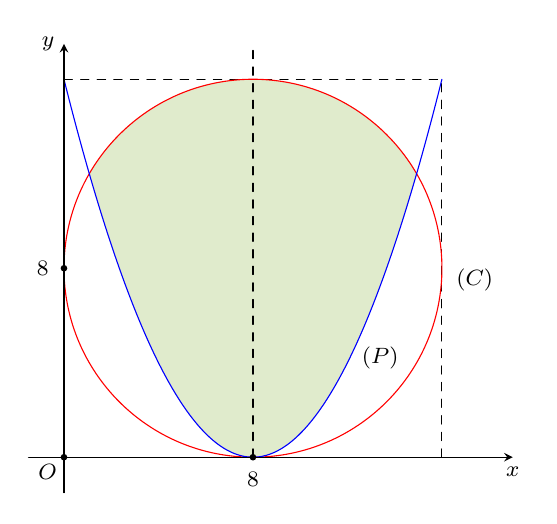
\begin{tikzpicture}[line cap=round, line join=round, >=stealth, scale=0.3, font=\footnotesize]
			\begin{scope}
				\clip (8,8) circle (8);
				\fill[green!20!olive!20] (0,17) -- plot[domain=0:16, smooth, samples=100] (\x, {0.25*(\x-8)^2}) -- (16,17) -- cycle;
			\end{scope}
			\draw[dashed] (8,0) -- (8,17.5) (16,0) -- (16,16)(0,16) -- (16,16);
			\draw[red] (8,8) circle (8);
			\draw[blue] plot[domain=0:16, smooth, samples=100] (\x, {0.25*(\x-8)^2});
			\draw[->] (-1.5, 0) -- (19, 0) node[below] {$x$};
			\draw[->] (0, -1.5) -- (0, 17.5) node[left] {$y$};
			\fill (0,0) circle (4pt) node[below left=-1pt] {$O$};
			\fill (8,0) circle (4pt) node[below=2pt] {$8$};
			\fill (0,8) circle (4pt) node[left=2pt] {$8$};
			\node[right] at (16.2, 7.5) {$(C)$};
			\node[right] at (12.2, 4.2) {$(P)$};
		\end{tikzpicture}
	}
	\par
	\shortans[0]{0,77}
	\loigiai{
		Hình tròn $(C)$ tiếp xúc với hai tia $Ox$, $Oy$ và có bán kính $R=8$ nên tâm của $(C)$ là $I(8;8)$.\\
		Phương trình hình tròn $(C)$ là $(x-8)^2 + (y-8)^2 \le 64$.\\
		Đặt $X = x-8$ và $Y = y-8$, điều kiện của $(C)$ trở thành $X^2 + Y^2 \le 64$.\\
		Số điểm có toạ độ nguyên thuộc $(C)$ là số các cặp số nguyên $(X;Y)$ thoả mãn $X^2 + Y^2 \le 64$.\\
		Ta liệt kê các giá trị của $X$:
		\begin{itemize}
			\item $X = 0 \Rightarrow Y^2 \le 64 \Rightarrow -8 \le Y \le 8$ (có $17$ giá trị).
			\item $X = \pm 1 \Rightarrow Y^2 \le 63 \Rightarrow -7 \le Y \le 7$ (có $15 \cdot 2 = 30$ giá trị).
			\item $X = \pm 2 \Rightarrow Y^2 \le 60 \Rightarrow -7 \le Y \le 7$ (có $15 \cdot 2 = 30$ giá trị).
			\item $X = \pm 3 \Rightarrow Y^2 \le 55 \Rightarrow -7 \le Y \le 7$ (có $15 \cdot 2 = 30$ giá trị).
			\item $X = \pm 4 \Rightarrow Y^2 \le 48 \Rightarrow -6 \le Y \le 6$ (có $13 \cdot 2 = 26$ giá trị).
			\item $X = \pm 5 \Rightarrow Y^2 \le 39 \Rightarrow -6 \le Y \le 6$ (có $13 \cdot 2 = 26$ giá trị).
			\item $X = \pm 6 \Rightarrow Y^2 \le 28 \Rightarrow -5 \le Y \le 5$ (có $11 \cdot 2 = 22$ giá trị).
			\item $X = \pm 7 \Rightarrow Y^2 \le 15 \Rightarrow -3 \le Y \le 3$ (có $7 \cdot 2 = 14$ giá trị).
			\item $X = \pm 8 \Rightarrow Y^2 \le 0 \Rightarrow Y = 0$ (có $1 \cdot 2 = 2$ giá trị).
		\end{itemize}
		Số phần tử của không gian mẫu là $n(\Omega) = 17 + 30 + 30 + 30 + 26 + 26 + 22 + 14 + 2 = 197$.\\
		Parabol $(P)$ có đỉnh $V(8;0)$ nên có phương trình dạng $y = a(x-8)^2$.\\
		Dựa vào hình vẽ, parabol đi qua điểm có toạ độ $(0;16)$ và $(16;16)$.\\
		Suy ra $16 = a(0-8)^2 \Leftrightarrow 64a = 16 \Leftrightarrow a = \dfrac{1}{4}$.\\
		Vậy phương trình $(P)$ là $y = \dfrac{1}{4}(x-8)^2$.\\
		Điểm thuộc phần tô màu là điểm thuộc $(C)$ và nằm phía trên hoặc trên parabol $(P)$.\\
		Toạ độ điểm $(x;y)$ phải thoả mãn hệ:
		\begin{eqnarray*} 
			\heva{&(x-8)^2 + (y-8)^2 \le 64 \\ &y \ge \dfrac{1}{4}(x-8)^2} &\Leftrightarrow& \heva{&X^2 + Y^2 \le 64 \\ &Y + 8 \ge \dfrac{1}{4}X^2} \\ 
			&\Leftrightarrow& \heva{&X^2 + Y^2 \le 64 \\ &Y \ge \dfrac{X^2}{4} - 8.} 
		\end{eqnarray*}
		Ta đếm số cặp số nguyên $(X;Y)$ thoả mãn hệ trên:
		\begin{itemize}
			\item $X = 0 \Rightarrow \heva{&Y^2 \le 64 \\ &Y \ge -8} \Rightarrow Y \in \{-8; -7; \dots; 8\}$ (có $17$ giá trị).
			\item $X = \pm 1 \Rightarrow \heva{&Y^2 \le 63 \\ &Y \ge -7{,}75} \Rightarrow Y \in \{-7; -6; \dots; 7\}$ (có $15 \cdot 2 = 30$ giá trị).
			\item $X = \pm 2 \Rightarrow \heva{&Y^2 \le 60 \\ &Y \ge -7} \Rightarrow Y \in \{-7; -6; \dots; 7\}$ (có $15 \cdot 2 = 30$ giá trị).
			\item $X = \pm 3 \Rightarrow \heva{&Y^2 \le 55 \\ &Y \ge -5{,}75} \Rightarrow Y \in \{-5; -4; \dots; 7\}$ (có $13 \cdot 2 = 26$ giá trị).
			\item $X = \pm 4 \Rightarrow \heva{&Y^2 \le 48 \\ &Y \ge -4} \Rightarrow Y \in \{-4; -3; \dots; 6\}$ (có $11 \cdot 2 = 22$ giá trị).
			\item $X = \pm 5 \Rightarrow \heva{&Y^2 \le 39 \\ &Y \ge -1{,}75} \Rightarrow Y \in \{-1; 0; \dots; 6\}$ (có $8 \cdot 2 = 16$ giá trị).
			\item $X = \pm 6 \Rightarrow \heva{&Y^2 \le 28 \\ &Y \ge 1} \Rightarrow Y \in \{1; 2; \dots; 5\}$ (có $5 \cdot 2 = 10$ giá trị).
			\item $X = \pm 7 \Rightarrow \heva{&Y^2 \le 15 \Rightarrow -3 \le Y \le 3 \\ &Y \ge 4{,}25}$ (không có giá trị $Y$ nguyên thoả mãn).
			\item $X = \pm 8 \Rightarrow \heva{&Y^2 \le 0 \Rightarrow Y = 0 \\ &Y \ge 8}$ (không có giá trị $Y$ nguyên thoả mãn).
		\end{itemize}
		Gọi $A$ là biến cố ``Điểm được chọn thuộc hình phẳng được tô màu''.\\
		Số kết quả thuận lợi cho $A$ là $n(A) = 17 + 30 + 30 + 26 + 22 + 16 + 10 = 151$.\\
		Xác suất cần tìm là $\mathrm{P}(A) = \dfrac{n(A)}{n(\Omega)} = \dfrac{151}{197} \approx 0{,}77$.
	}
\end{ex}

\begin{ex}%[1D3V3-5]%[TDM42]
	Có hai hộp đựng các viên bi cùng kích thước và khối lượng. Hộp I có $5$ bi đỏ và $3$ bi xanh, hộp II có $4$ bi đỏ và $3$ bi xanh. Gieo ngẫu nhiên một con xúc xắc cân đối đồng chất hai lần liên tiếp. Trong mỗi lần nếu số chấm nhỏ hơn $5$ thì lấy ngẫu nhiên ba viên bi từ hộp I bỏ sang hộp II, nếu số chấm lớn hơn $4$ thì lấy ngẫu nhiên ba viên bi từ hộp II bỏ sang hộp I. Biết xác suất để hộp I vẫn có đủ hai màu, nếu biết số bi ở hộp I vẫn là $8$ viên là $\dfrac{b}{10\,000}$. Hãy tính $b$ (làm tròn kết quả đến hàng đơn vị)?
	\par
	\shortans[0]{9994}
	\loigiai{
		Gọi $C$ là biến cố ``Gieo con xúc xắc được số chấm nhỏ hơn $5$''. Ta có $\mathrm{P}(C) = \dfrac{4}{6} = \dfrac{2}{3}$ và $\mathrm{P}(\overline{C}) = \dfrac{2}{6} = \dfrac{1}{3}$.\\
		Gọi $B$ là biến cố ``Số bi ở hộp I vẫn là $8$ viên sau hai lần gieo xúc xắc''. Điều này xảy ra khi và chỉ khi có đúng $1$ lần chuyển bi từ hộp I sang hộp II (tương ứng với biến cố $C$) và $1$ lần chuyển bi từ hộp II sang hộp I (tương ứng với biến cố $\overline{C}$).
		\[ \mathrm{P}(B) = \mathrm{P}(C) \cdot \mathrm{P}(\overline{C}) + \mathrm{P}(\overline{C}) \cdot \mathrm{P}(C) = \dfrac{4}{6} \cdot \dfrac{2}{6} + \dfrac{2}{6} \cdot \dfrac{4}{6} = \dfrac{16}{36} = \dfrac{4}{9} \]
		Gọi $A$ là biến cố ``Hộp I vẫn có đủ hai màu''. Theo đề bài ta cần tính xác suất có điều kiện:
		\[ \mathrm{P}(A|B) = 1 - \mathrm{P}(\overline{A}|B) = 1 - \dfrac{\mathrm{P}(\overline{A}B)}{\mathrm{P}(B)} \]
		Biến cố $\overline{A}B$ là ``Hộp I có $8$ viên bi nhưng không đủ hai màu''. Tổng số bi xanh của cả hai hộp là $6$ bi nên hộp I không thể chứa toàn $8$ bi xanh. Vậy để xảy ra $\overline{A}B$ thì hộp I phải chứa đúng $8$ bi đỏ.\\
		Có $2$ trường hợp xảy ra cho biến cố $\overline{A}B$:
		\begin{enumerate}[\it TH 1:]
			\item Lần 1 gieo $<5$ (chuyển $3$ bi từ I sang II), lần 2 gieo $>4$ (chuyển $3$ bi từ II sang I).\\
			Để hộp I chỉ còn bi đỏ, lần 1 phải chuyển $3$ bi xanh từ I sang II; khi đó hộp II sẽ có $4$ đỏ, $6$ xanh. Lần 2 phải chuyển $3$ bi đỏ từ II sang I.\\
			Xác suất xảy ra trường hợp này là:
			\[ P_1 = \dfrac{4}{6} \cdot \dfrac{\mathrm{C}_3^3}{\mathrm{C}_8^3} \cdot \dfrac{2}{6} \cdot \dfrac{\mathrm{C}_4^3}{\mathrm{C}_{10}^3} = \dfrac{4}{6} \cdot \dfrac{1}{56} \cdot \dfrac{2}{6} \cdot \dfrac{4}{120} = \dfrac{1}{7\,560} \]
			\item Lần 1 gieo $>4$ (chuyển $3$ bi từ II sang I), lần 2 gieo $<5$ (chuyển $3$ bi từ I sang II).\\
			Để hộp I cuối cùng chỉ còn bi đỏ, lần 1 phải chuyển $3$ bi đỏ từ II sang I; khi đó hộp I sẽ có $8$ đỏ, $3$ xanh. Lần 2 phải chuyển $3$ bi xanh từ I sang II.\\
			Xác suất xảy ra trường hợp này là:
			\[ P_2 = \dfrac{2}{6} \cdot \dfrac{\mathrm{C}_4^3}{\mathrm{C}_7^3} \cdot \dfrac{4}{6} \cdot \dfrac{\mathrm{C}_3^3}{\mathrm{C}_{11}^3} = \dfrac{2}{6} \cdot \dfrac{4}{35} \cdot \dfrac{4}{6} \cdot \dfrac{1}{165} = \dfrac{8}{51\,975} \]
		\end{enumerate}
		Suy ra $\mathrm{P}(\overline{A}B) = P_1 + P_2 = \dfrac{1}{7\,560} + \dfrac{8}{51\,975} = \dfrac{17}{59\,400}$.\\
		Vậy xác suất cần tìm là:
		\[ \mathrm{P}(A|B) = 1 - \dfrac{17/59\,400}{4/9} = 1 - \dfrac{17}{26\,400} = \dfrac{26\,383}{26\,400} \approx 0{,}999356 \]
		Theo giả thiết $\dfrac{b}{10\,000} \approx 0{,}999356 \Rightarrow b \approx 9\,993{,}56$.\\
		Làm tròn kết quả đến hàng đơn vị, ta được $b = 9\,994$.
	}
\end{ex}

\begin{ex}%[2H3C2-3]%[TDM32]%[Nguyễn Văn Sang]
	Trong không gian $Oxyz$ có đơn vị dài trên mỗi trục là centimet, cho ba điểm $A(100;0;0)$, $B(64;24;-24\sqrt3)$, $C(64;-24;24\sqrt3)$. Gọi đường tròn $(C)$ là tập hợp các điểm $M$ thỏa mãn $MO=80$, $MA=60$. Gọi $(H)$ là tập hợp các điểm $N$ nằm trong hình tròn $(C)$ và thỏa mãn $NB+NC\le 120$. Hãy tính theo đơn vị $\text{dm}^2$ diện tích hình phẳng $(H)$ \textit{(không làm tròn ở các phép tính trung gian và làm tròn kết quả cuối cùng đến hàng phần mười)}.
	\par
	\shortans[0]{58,8}
	\loigiai{
		Giả sử điểm $M(x;y;z)$ thuộc đường tròn $(C)$. Theo giả thiết ta có hệ phương trình:
		\begin{eqnarray*} 
			\heva{& x^2 + y^2 + z^2 = 80^2 = 6\,400 \\ & (x-100)^2 + y^2 + z^2 = 60^2 = 3\,600} &\Rightarrow& x^2 - (x-100)^2 = 2\,800 \\ 
			&\Leftrightarrow& 200x - 10\,000 = 2\,800 \\ 
			&\Leftrightarrow& x = 64. 
		\end{eqnarray*}
		Thay $x = 64$ vào phương trình đầu, ta được $y^2 + z^2 = 6\,400 - 64^2 = 2\,304 = 48^2$.\\
		Vậy $(C)$ là đường tròn nằm trong mặt phẳng $(\alpha)\colon x = 64$, có tâm $I(64;0;0)$ và bán kính $R = 48$.\\
		Hai điểm $B, C$ đều có hoành độ $x=64$ nên cùng thuộc mặt phẳng $(\alpha)$.\\
		Ta có $\overrightarrow{IB} = (0;24;-24\sqrt3)$ và $\overrightarrow{IC} = (0;-24;24\sqrt3) = -\overrightarrow{IB}$. Điểm $I$ là trung điểm của đoạn thẳng $BC$.\\
		Độ dài $IB = IC = \sqrt{24^2 + (-24\sqrt3)^2} = 48 = R$. Suy ra $B, C$ là hai điểm nằm trên đường tròn $(C)$.\\
		Tập hợp các điểm $N$ thuộc mặt phẳng $(\alpha)$ thỏa mãn $NB + NC \le 120$ là miền trong (tính cả biên) của elip $(E)$ có hai tiêu điểm $B$ và $C$.\\
		Xét các thông số của elip $(E)$:
		\begin{itemize}
			\item Độ dài trục lớn: $2a = 120 \Rightarrow a = 60$.
			\item Tiêu cự: $2c = BC = 2 \cdot 48 = 96 \Rightarrow c = 48$.
			\item Độ dài bán trục bé: $b = \sqrt{a^2 - c^2} = \sqrt{60^2 - 48^2} = 36$.
		\end{itemize}
		\begin{center}
			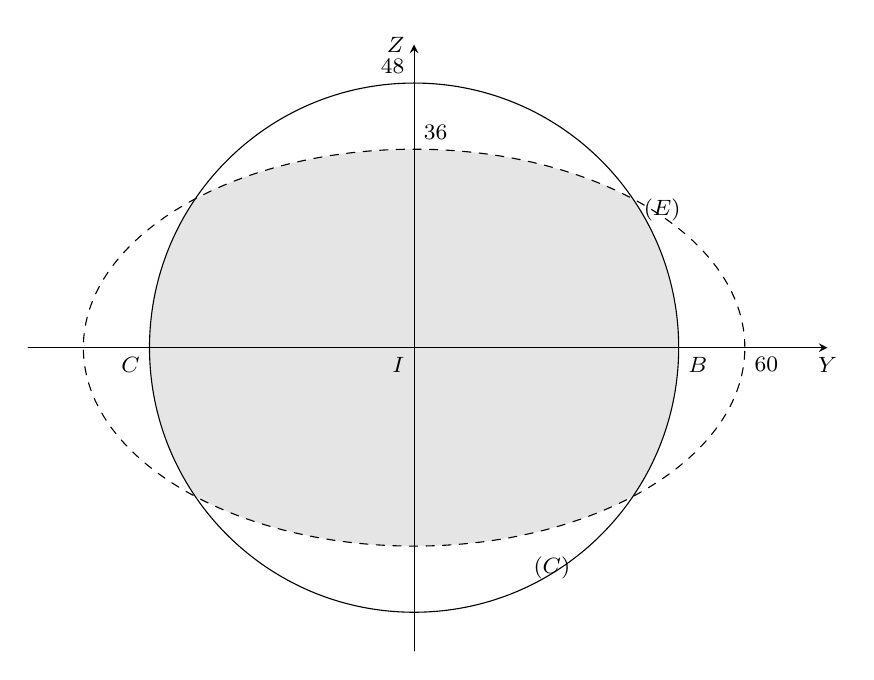
\begin{tikzpicture}[scale=0.07, font=\footnotesize, line join=round, line cap=round, >=stealth]
				% Tô màu phần giao nhau (H)
				\begin{scope}
					\clip (0,0) circle (48);
					\fill[gray!20] (0,0) ellipse (60 and 36);
				\end{scope}
				
				% Vẽ elip (E) và hình tròn (C)
				\draw[dashed] (0,0) ellipse (60 and 36);
				\draw (0,0) circle (48);
				
				% Trục tọa độ
				\draw[->] (-70,0) -- (75,0) node[below] {$Y$};
				\draw[->] (0,-55) -- (0,55) node[left] {$Z$};
				
				% Các điểm và Ghi chú
				\fill (0,0) circle (1.5pt) node[below left] {$I$};
				\fill (48,0) circle (1.5pt) node[below right] {$B$};
				\fill (-48,0) circle (1.5pt) node[below left] {$C$};
				\fill (60,0) circle (1.5pt) node[below right] {$60$};
				\fill (0,36) circle (1.5pt) node[above right] {$36$};
				\fill (0,48) circle (1.5pt) node[above left] {$48$};
				
				\node at (25, -40) {$(C)$};
				\node at (45, 25) {$(E)$};
			\end{tikzpicture}
		\end{center}
		Gắn hệ trục tọa độ $IYZ$ trên mặt phẳng $(\alpha)$ sao cho gốc tọa độ trùng với $I$, tia $IY$ chứa điểm $C$. Khi đó ta có phương trình:
		\begin{itemize}
			\item Đường tròn $(C)\colon Y^2 + Z^2 = 48^2$.
			\item Elip $(E)\colon \dfrac{Y^2}{60^2} + \dfrac{Z^2}{36^2} = 1$.
		\end{itemize}
		Tập hợp $(H)$ là phần giao của hình tròn $(C)$ và elip $(E)$. Xét trong góc phần tư thứ nhất của hệ $IYZ$, hoành độ giao điểm của $(C)$ và $(E)$ là nghiệm của hệ:
		\[ \heva{& Y^2 + Z^2 = 2\,304 \\ & \dfrac{Y^2}{3\,600} + \dfrac{Z^2}{1\,296} = 1} \Rightarrow \dfrac{Y^2}{3\,600} + \dfrac{2\,304 - Y^2}{1\,296} = 1 \Leftrightarrow Y^2 = 1\,575 \Rightarrow Y = 15\sqrt{7} \]
		Do tính đối xứng, phần diện tích hình tròn $(C)$ nằm \textbf{ngoài} elip $(E)$ gồm $4$ hình chỏm bằng nhau. Diện tích $4$ chỏm này là:
		\[ S_{\text{ngoài}} = 4 \displaystyle\int\limits_0^{15\sqrt{7}} \left( \sqrt{48^2 - Y^2} - 36\sqrt{1 - \dfrac{Y^2}{60^2}} \right) \mathrm{\,d}Y \]
		Sử dụng công thức nguyên hàm $\displaystyle\int \sqrt{r^2 - u^2} \mathrm{\,d}u = \dfrac{u}{2}\sqrt{r^2-u^2} + \dfrac{r^2}{2}\arcsin\dfrac{u}{r}$, ta có:
		\begin{align*} 
			\displaystyle\int\limits_0^{15\sqrt{7}} \sqrt{48^2 - Y^2} \mathrm{\,d}Y &= \dfrac{405\sqrt{7}}{2} + 1\,152\arcsin\dfrac{5\sqrt{7}}{16} \\ 
			36 \displaystyle\int\limits_0^{15\sqrt{7}} \sqrt{1 - \dfrac{Y^2}{60^2}} \mathrm{\,d}Y &= \dfrac{36}{60} \displaystyle\int\limits_0^{15\sqrt{7}} \sqrt{60^2 - Y^2} \mathrm{\,d}Y = \dfrac{405\sqrt{7}}{2} + 1\,080\arcsin\dfrac{\sqrt{7}}{4} 
		\end{align*}
		Suy ra:
		\[ S_{\text{ngoài}} = 4 \left( 1\,152\arcsin\dfrac{5\sqrt{7}}{16} - 1\,080\arcsin\dfrac{\sqrt{7}}{4} \right) \approx 1\,363{,}18 \,(\text{cm}^2) \]
		Diện tích hình phẳng $(H)$ là:
		\[ S_{(H)} = S_{(C)} - S_{\text{ngoài}} = \pi \cdot 48^2 - S_{\text{ngoài}} \approx 7\,238{,}23 - 1\,363{,}18 = 5\,875{,}05 \,(\text{cm}^2) = 58{,}75 \,(\text{dm}^2) \]
		Làm tròn kết quả đến hàng phần mười, ta được $58{,}8$\,dm$^2$.
	}
\end{ex}